\chapterold{GOTO operator}

The GOTO operator is generally considered as anti-pattern, see
[Edgar Dijkstra, \IT{Go To Statement Considered Harmful} (1968)\footnote{\url{http://yurichev.com/mirrors/Dijkstra68.pdf}}].
Nevertheless, it can be used reasonably, see 
[Donald E. Knuth, \IT{Structured Programming with go to Statements} (1974)\footnote{\url{http://yurichev.com/mirrors/KnuthStructuredProgrammingGoTo.pdf}}]
\footnote{[\CNotes] also has some examples.}.

Here is a very simple example:

\lstinputlisting{patterns/065_GOTO/goto.c}

Here is what we have got in MSVC 2012:

\lstinputlisting[caption=MSVC 2012]{patterns/065_GOTO/MSVC_goto.asm}

The \IT{goto} statement has been simply replaced by a \JMP instruction, which has the same effect: unconditional jump to another place.
The second \printf could be executed only with human intervention, by using a debugger or by patching the code.

\par

\clearpage

This could also be useful as a simple patching exercise. Let's open the resulting executable in Hiew:

\begin{figure}[H]
\centering
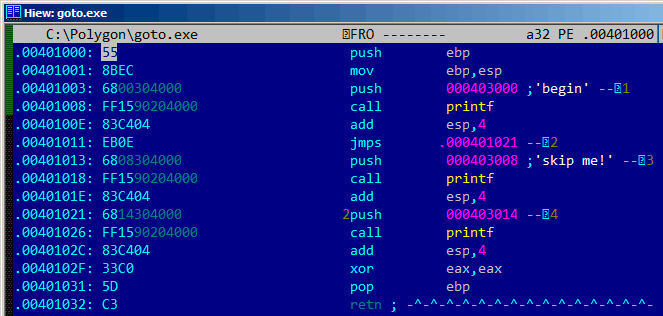
\includegraphics[scale=\FigScale]{patterns/065_GOTO/hiew1.png}
\caption{Hiew}
\label{fig:goto_hiew1}
\end{figure}

\clearpage
Place the cursor to address \JMP (\TT{0x410}), 
press F3 (edit), press zero twice, so the opcode becomes \TT{EB 00}:

\begin{figure}[H]
\centering
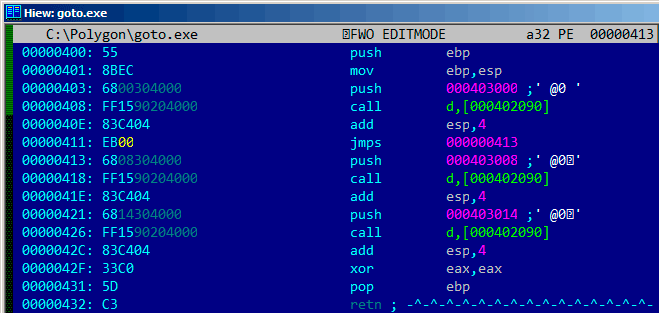
\includegraphics[scale=\FigScale]{patterns/065_GOTO/hiew2.png}
\caption{Hiew}
\label{fig:goto_hiew2}
\end{figure}

The second byte of the \JMP opcode denotes the relative offset for the jump, 0 means the point
right after the current instruction.

So now \JMP not skipping the second \printf call.

Press F9 (save) and exit.  Now if we run the executable we should see this:

\begin{figure}[H]
\centering
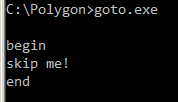
\includegraphics[scale=\NormalScale]{patterns/065_GOTO/result.png}
\caption{Patched executable output}
\label{fig:goto_result}
\end{figure}

The same result could be achieved by replacing the \JMP instruction with 2 \NOP instructions.

\NOP has an opcode of \TT{0x90} and length of 1 byte, so we need 2 instructions as \JMP replacement (which is 2 bytes in size).

\sectionold{Dead code}

The second \printf call is also called \q{dead code} in compiler terms.

This means that the code will never be executed.
So when you compile this example with optimizations, the compiler removes \q{dead code}, leaving
no trace of it:

\lstinputlisting[caption=\Optimizing MSVC 2012]{patterns/065_GOTO/MSVC_goto_Ox.asm}

However, the compiler forgot to remove the \q{skip me!} string.

%Note: cl "/Ox" option for maximum optimisation does get rid of "skip me" string as well

\sectionold{\Exercise}

% TODO debugger example can fit here

Try to achieve the same result using your favorite compiler and debugger.

